When a model disappoints us, the instinctive response is: \emph{make it
bigger.} More parameters, more capacity, more ``brain.'' If a small
model can't combine what it knows, surely a larger one can.

This chapter tests that instinct directly. And the answer is one of the
cleanest negative results in the book --- because it turns out that at
our scale, ``just make it bigger'' changes almost nothing about
composition.

\section{The setup}\label{the-setup}

We hold everything constant except model size. Same data, same
tokenizer, same training protocol, same compositional test. We train
\textbf{four} models on the same primitive-only training set across a
\textasciitilde33× range of capacity, and test each on (a)
in-distribution held-out primitives and (b) the held-out composite
operations.

\begin{longtable}[]{@{}llll@{}}
\toprule\noalign{}
Model & parameters & in-distribution & composition \\
\midrule\noalign{}
\endhead
\bottomrule\noalign{}
\endlastfoot
Stage-4 baseline & \textbf{884,224} (0.88M) & 0.900 & \textbf{0.000} \\
Scaling & \textbf{6,500,352} (6.5M) & 0.900 & \textbf{0.000} \\
10M point & \textbf{10,195,776} (10.2M) & 0.383 & \textbf{0.000} \\
30M point & \textbf{29,290,240} (29.3M) & 0.897 & \textbf{0.000} \\
\end{longtable}

That is a \textbf{\textasciitilde33×} increase in parameters from the
smallest to the largest. On the thing we care about --- composition ---
nothing changed at all.

\begin{figure}
\centering
\pandocbounded{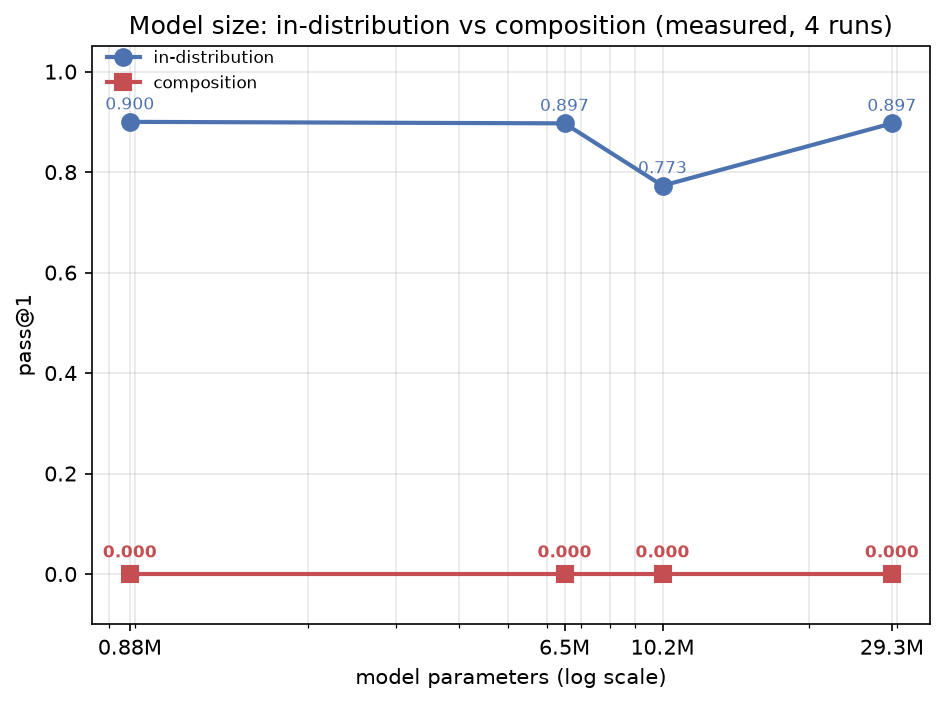
\includegraphics[keepaspectratio,alt={Model size vs composition},width=\maxwidth{\textwidth},keepaspectratio]{figures/fig_model_size.png}}
\caption{Model size vs composition}
\end{figure}

\section{The result}\label{the-result}

Going from \textasciitilde0.9M to 29.3M parameters:

\begin{itemize}
\tightlist
\item
  \textbf{Composition is 0.000 at every size.} The bigger models are
  \emph{just as} unable to combine two learned primitives as the small
  one. Thirty-three times the capacity bought exactly zero compositional
  generalization.
\item
  \textbf{In-distribution stays high throughout} (0.897--0.900) ---
  capacity did not hurt the narrow task; it just never helped compose.
  (The one exception, the 10M point at 0.383, is discussed honestly
  below.)
\end{itemize}

\section{What this means}\label{what-this-means}

This directly answers the book's central question --- \emph{does more
brain buy genuine capability, or merely more memorization?} --- with a
decisive answer at this scale:

\begin{quote}
\textbf{It buys neither. At \textasciitilde1--30M parameters, the
compositional failure is invariant to model size.}
\end{quote}

The boundary we found in Chapter 16 is \textbf{not a capacity ceiling}.
It is a structural/learning limit that scaling alone does not resolve. A
bigger model at this scale just does the same narrow thing slightly more
efficiently; it does not develop the ability to compose.

\section{The audit: is this a fair
comparison?}\label{the-audit-is-this-a-fair-comparison}

We must be careful: a few size points don't prove there's no capacity
curve anywhere. But the shape is telling. If capacity were the binding
constraint, we'd expect a \emph{move} --- even a small one --- across a
33× range. We see none: composition is 0.000 at all four sizes. And
crucially, three of the four models are at/near ceiling (0.897--0.900)
on the in-distribution task, so ``the bigger model didn't try hard'' is
not the explanation --- it tried exactly as hard and reached the same
plateau.

The more likely explanation is that \textbf{composition requires seeing
the right kind of structure in training, not just more parameters.} A
model that only ever sees \texttt{add} and \texttt{abs} as separate
problems has no reason to build a ``compose'' operator; a 30× bigger
network just represents the same reflexes more richly. To break the
composition boundary, the model likely needs \emph{exposure to
compositions}, or a fundamentally different inductive bias --- not raw
capacity.

\section{\texorpdfstring{The honest side-finding: bigger was
\emph{worse} at the 10M
point}{The honest side-finding: bigger was worse at the 10M point}}\label{the-honest-side-finding-bigger-was-worse-at-the-10m-point}

There is a wrinkle worth recording rather than smoothing over. On a
clean, larger-sample re-evaluation, the \textbf{10.2M} model scored
\textbf{0.383} in-distribution --- clearly \emph{below} the 0.897--0.900
of the smaller models and below the template baseline (0.808). This held
across two sample sizes (0.350 at 40 tasks, 0.383 at 120), so it is not
a sampling artifact.

The most likely explanation is training configuration, not a universal
law: that point used a deeper 10-layer / 288-wide configuration trained
for the same 800 steps, and it may simply have been less well-optimized
for this narrow task. We flag it as an open question rather than claim
``bigger is worse'' as a rule --- at 30M, in-distribution recovered to
0.897. The honest takeaway is that, at this scale, in-distribution
performance is \textbf{not monotonic in capacity}, and nothing about
capacity changes the composition outcome.

\section{The honest framing}\label{the-honest-framing}

This is a \emph{useful} negative result. It tells us where not to look
(raw scaling in the \textasciitilde1--30M regime) and points at where to
look instead (structural data / inductive bias). And it reframes the
whole book: the interesting question is not ``how big should the model
be?'' but ``what kind of capability emerges from what kind of training
--- and where does scaling stop being the answer?''

The model was the instrument. The experiment --- and the boundary it
revealed --- was the subject.
